\section{Durchführung}
Es wurden ein Oszilloskop und eine Spannungsquelle zur Verfügung gestellt.

\subsection{Aufgabe a)}
Um die Zeitkonstante zu bestimmen, wird das Experiment nach Abbildung (\ref{fig:rcaa}) aufgebaut.

\begin{figure}
            \centering
               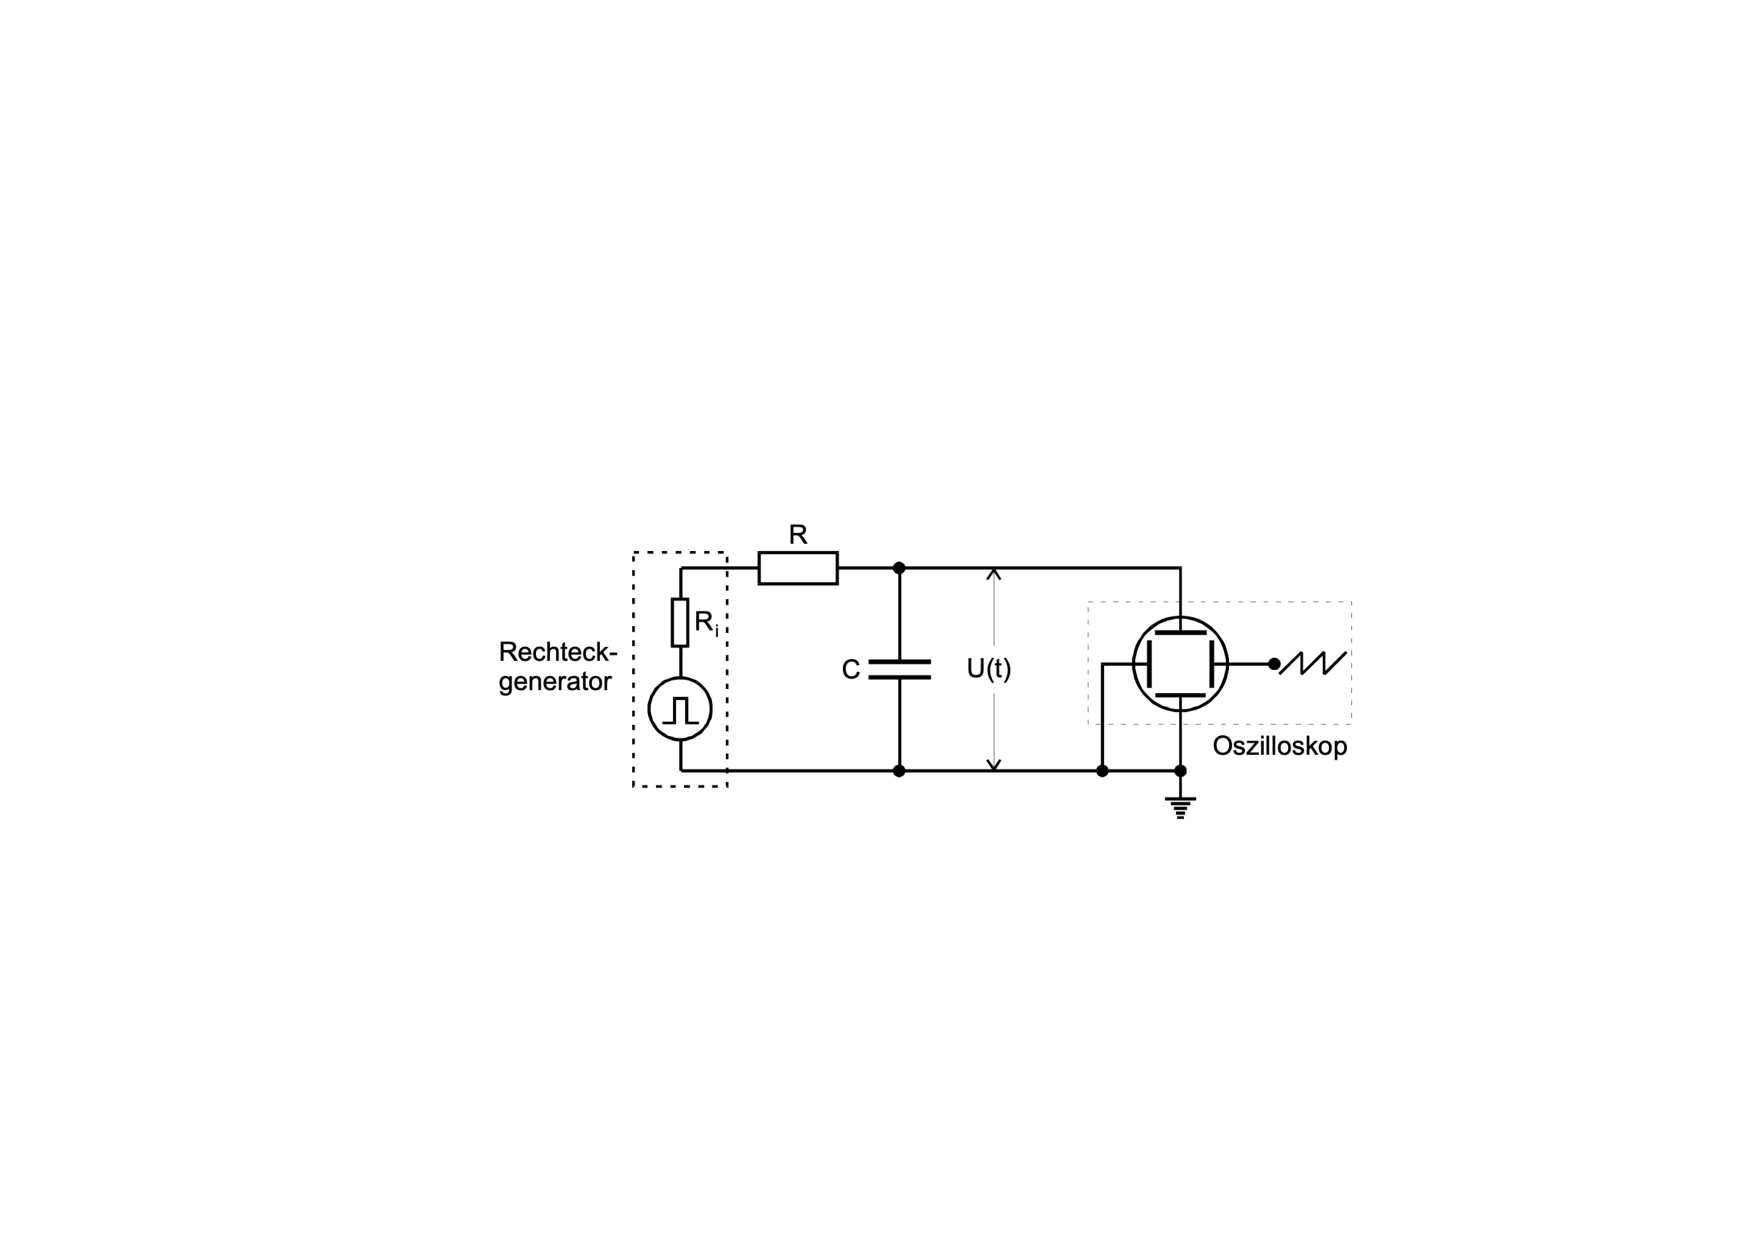
\includegraphics[height=5cm]{rcaa.pdf}
               \caption{Aufbau zur Bestimmung der Zeitkonstante.}
               \label{fig:rcaa}
\end{figure}

\noindent
Mithilfe des Oszilloskops wird die Kondensatorspannung in Abhängigkeit von der Zeit graphisch dargestellt und ein geeigneter Ausschnitt der Entladekurve betrachtet.
Mit dem Cursor werden nun verschiedene Punkte auf der Kurve eingelesen.
Diese wurden vermessen, notiert und in Tabelle (\ref{tab:a}) aufgeführt.

\subsection{Aufgabe b)}
Die Abhängigkeit der Kondensatorspannungsamplitude von der Frequenz kann mit dem in Abbildung (\ref{fig:rcab}) dargestellten Aufbau untersucht werden.

\begin{figure}
            \centering
               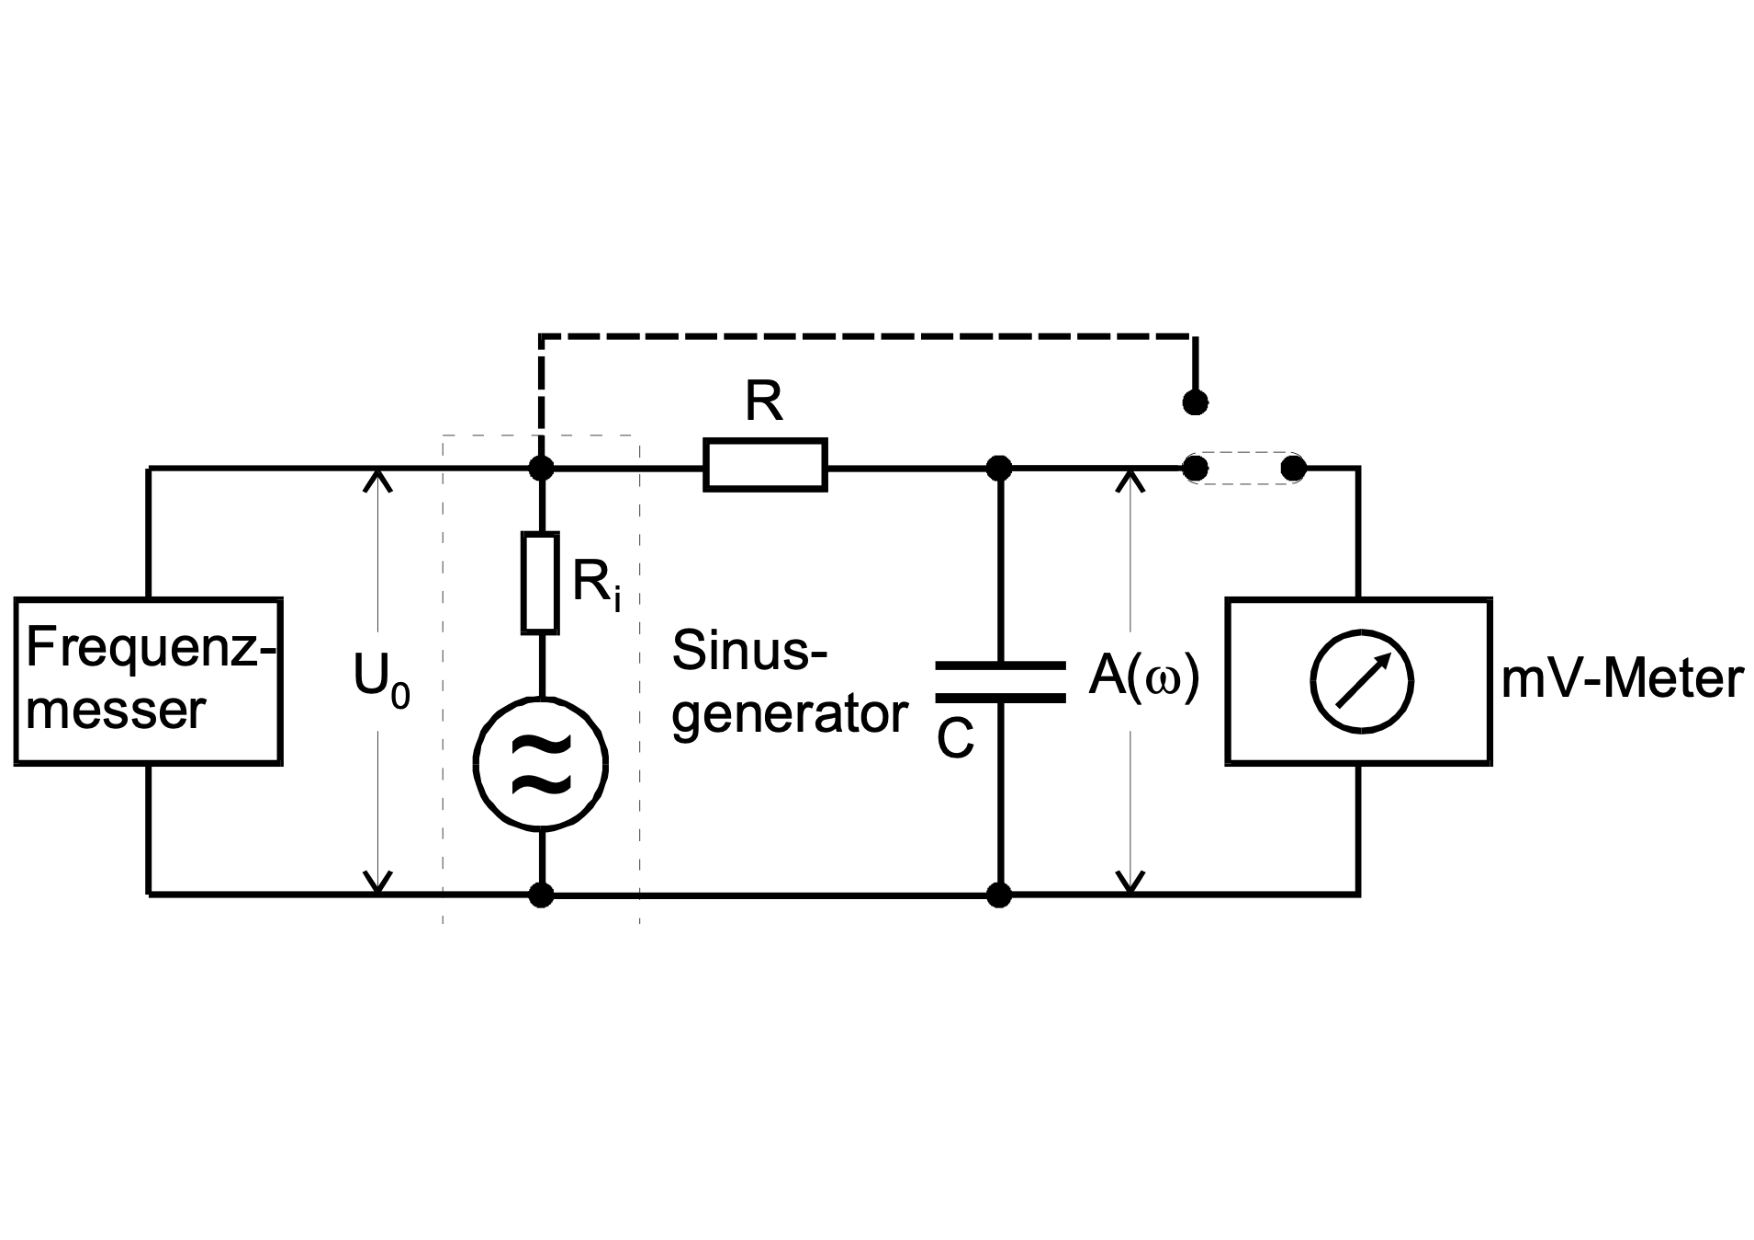
\includegraphics[height=4.5cm]{rcab.pdf}
               \caption{Aufbau zur Untersuchung der Abhängigkeit der Kondensatorspannungsamplitude von der Frequenz.}
               \label{fig:rcab}
\end{figure}

\noindent
Dazu wird der Spannungsverlauf auf dem Oszilloskop betrachtet und mit dem Cursor vermessen, wobei die Frequenz verändert wird.
Die Kondensatorspannungsamplituden werden in Abhängigkeit von verschiedenen Frequenzen $10\si{\hertz} < \text{f} < 5\si{\kilo\hertz}$ vermessen, notiert und in Tabelle (\ref{tab:b}) aufgeführt.

\subsection{Aufgabe c)}
Um die Phasenverschiebung $\phi$ zwischen der Generatorspannung und der Kondensatorspannung zu messen, kann der Versuch nach Abbildung (\ref{fig:rcac}) aufgebaut werden.

\newpage
\begin{figure}
            \centering
               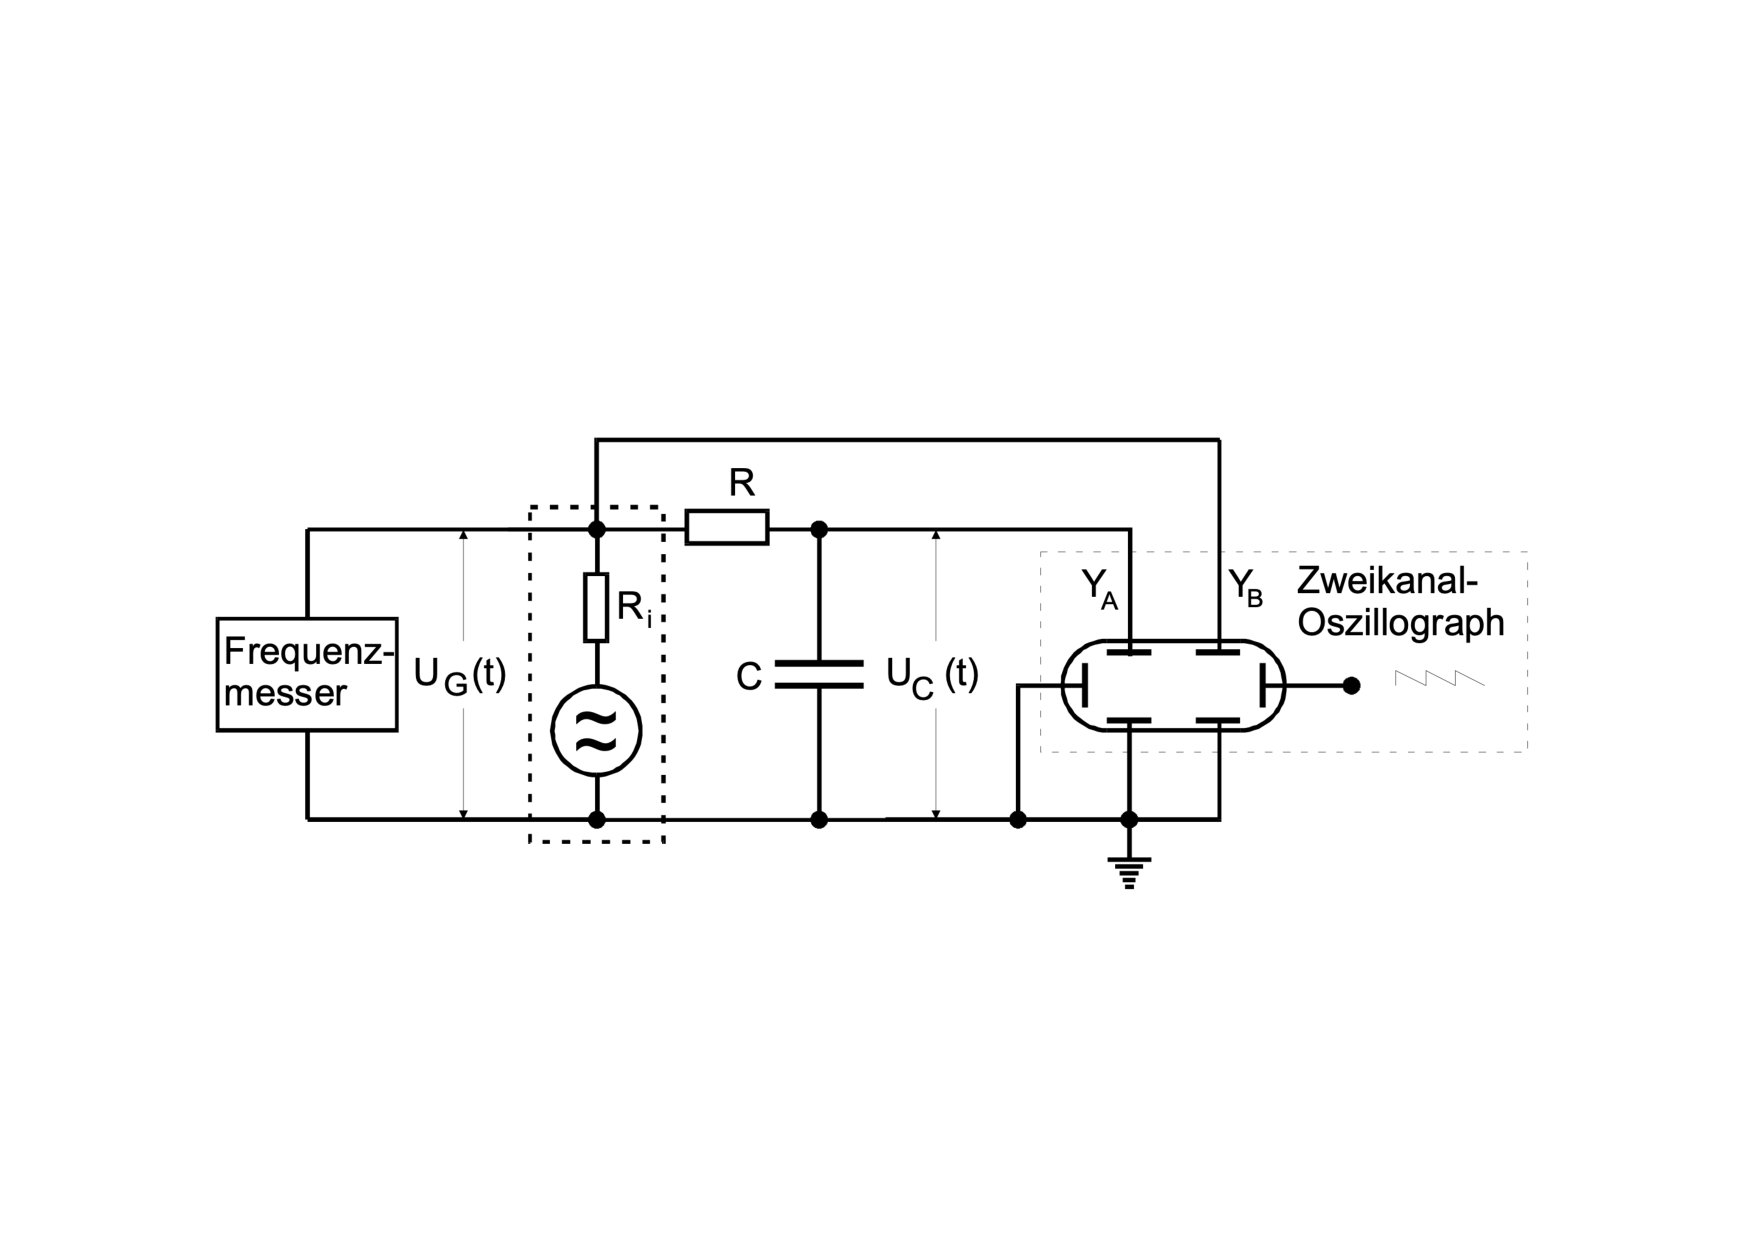
\includegraphics[height=5cm]{rcac.pdf}
               \caption{Aufbau zur Bestimmung der Phasenverschiebung.}
               \label{fig:rcac}
\end{figure}

\noindent
Nun können am Oszilloskop beide Spannungsverläufe gleichzeitig beobachtet werden.
Diese werden ähnlich zur Abbildung (\ref{fig:rcac2}) auf dem Oszilloskop dargestellt:

\begin{figure}
            \centering
               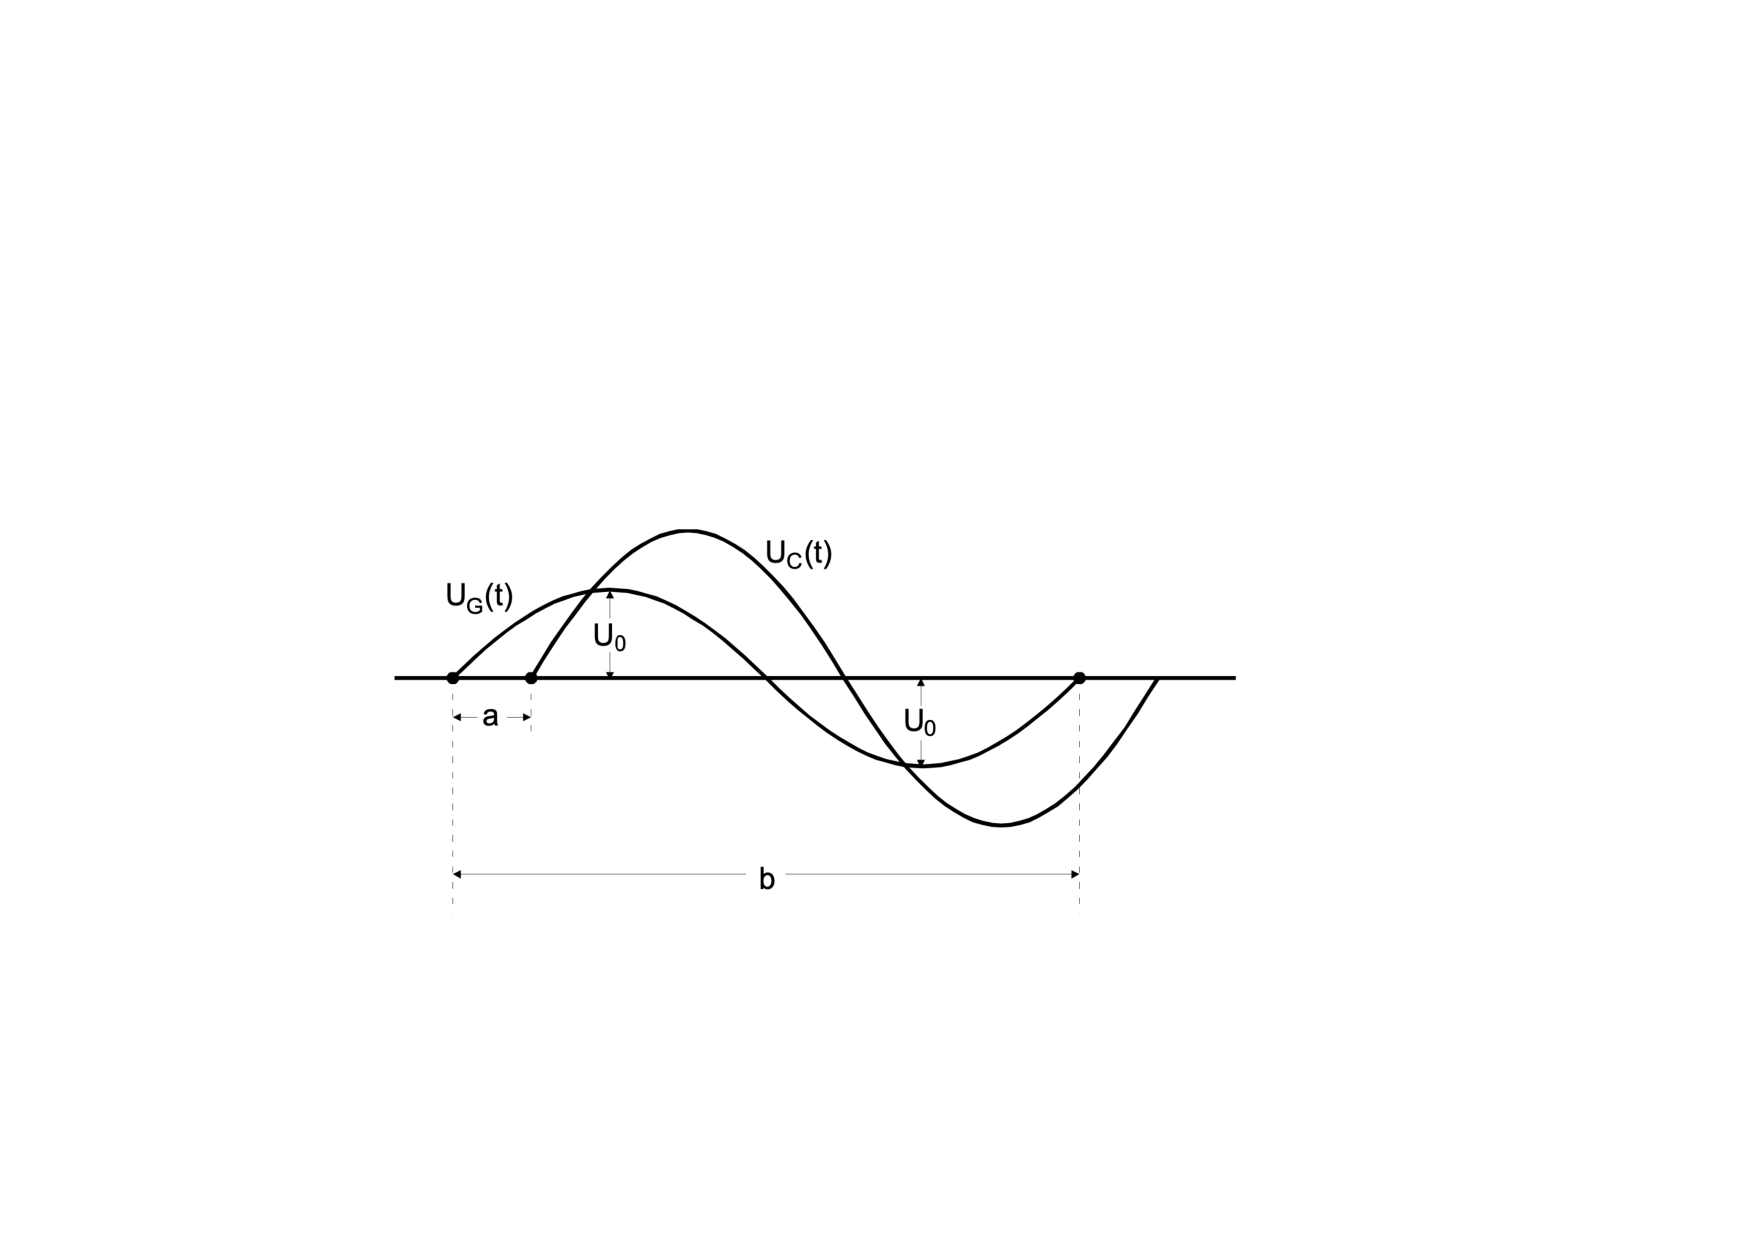
\includegraphics[height=5cm]{rcac2.pdf}
               \caption{Form der beiden Spannungsverläufe am Oszilloskop.}
               \label{fig:rcac2}
\end{figure}

\noindent
Die Wellenlänge a sowie die Schwingungsdauer b werden für verschiedene Frequenzen mit dem Cursor vermessen, notiert und in Tabelle (\ref{tab:c}) aufgeführt. 

\subsection{Aufgabe d)}
Um zu zeigen dass ein RC-Kreis auch als Integrator arbeiten kann, wird die Schaltung in Abbildung (\ref{fig:rcac}) verwendet.
Nun wird nacheinander eine Rechteck-, Sinus- und Dreiecksspannung auf das RC-Glied gegeben von dessen Verlauf auf dem Oszilloskop jeweils ein Foto gemacht wird. 
